\documentclass[tikz,border=7pt]{standalone}
\usepackage{amsmath,amssymb}
\usetikzlibrary{arrows.meta,calc,positioning,decorations.pathreplacing}

% ============================================================
% Three explicit, sphere-specialized pictures at p = (0,0,1):
%   (1) Gauss map  N:S^2->S^2,  p |-> p
%   (2) Differential (dN)_p : T_p S^2 -> T_{N(p)} S^2  with (dN)_p(v)=v
%   (3) Shape operator S_p = -(dN)_p : T_p S^2 -> T_p S^2 with S_p(v)=-v
%
% All drawings are in the xz cross-section (y=0), where:
%   S^2 ∩ {y=0} is the unit circle x^2+z^2=1,
%   p = (0,1) in this cross-section,
%   v corresponds to (1,0,0) (drawn as (1,0) in the cross-section).
% ============================================================

\begin{document}
	
	% ============================================================
	% (1) Gauss map N: S^2 -> S^2, N(p)=p  (identity map)
	% ============================================================
	\begin{tikzpicture}[>=Latex, line cap=round, line join=round, scale=3.8]
		
		% Left sphere (as unit circle in xz-plane)
		\begin{scope}[shift={(0,0)}]
			\draw[thick] (0,0) circle (1);
			\node at (0,1.28) {$S^2$ (domain)};
			% axes
			\draw[->] (-1.15,0) -- (1.15,0) node[below] {$x$};
			\draw[->] (0,-0.15) -- (0,1.35) node[left] {$z$};
			
			% point p (north pole)
			\coordinate (pL) at (0,1);
			\fill (pL) circle (0.9pt) node[above left] {$p=(0,0,1)$};
			
			% outward normal N(p)=p (radial)
			\draw[very thick,->] (pL) -- ++(0,0.35) node[above] {$N(p)$};
			
			% label N(p)=p
			\node[align=left] at (-1.13,0.75) {$N:S^2\to S^2$\\[-2pt] $p\mapsto p$};
		\end{scope}
		
		% Right sphere (codomain)
		\begin{scope}[shift={(3.1,0)}]
			\draw[thick] (0,0) circle (1);
			\node at (0,1.28) {$S^2$ (codomain)};
			% axes
			\draw[->] (-1.15,0) -- (1.15,0) node[below] {$x$};
			\draw[->] (0,-0.15) -- (0,1.35) node[left] {$z$};
			
			% point N(p)=p in codomain
			\coordinate (pR) at (0,1);
			\fill (pR) circle (0.9pt) node[above right] {$N(p)=p$};
			
			% radial arrow from origin to N(p)
			\draw[->] (0,0) -- (pR);
		\end{scope}
		
		% Map arrow N
		\draw[very thick,->] (1.15,1.02) -- (1.95,1.02) node[midway, above] {$N$};
		
	\end{tikzpicture}
	
	\vspace{10pt}
	
	% ============================================================
	% (2) Differential (dN)_p : T_p S^2 -> T_{N(p)} S^2, and (dN)_p(v)=v
	% ============================================================
	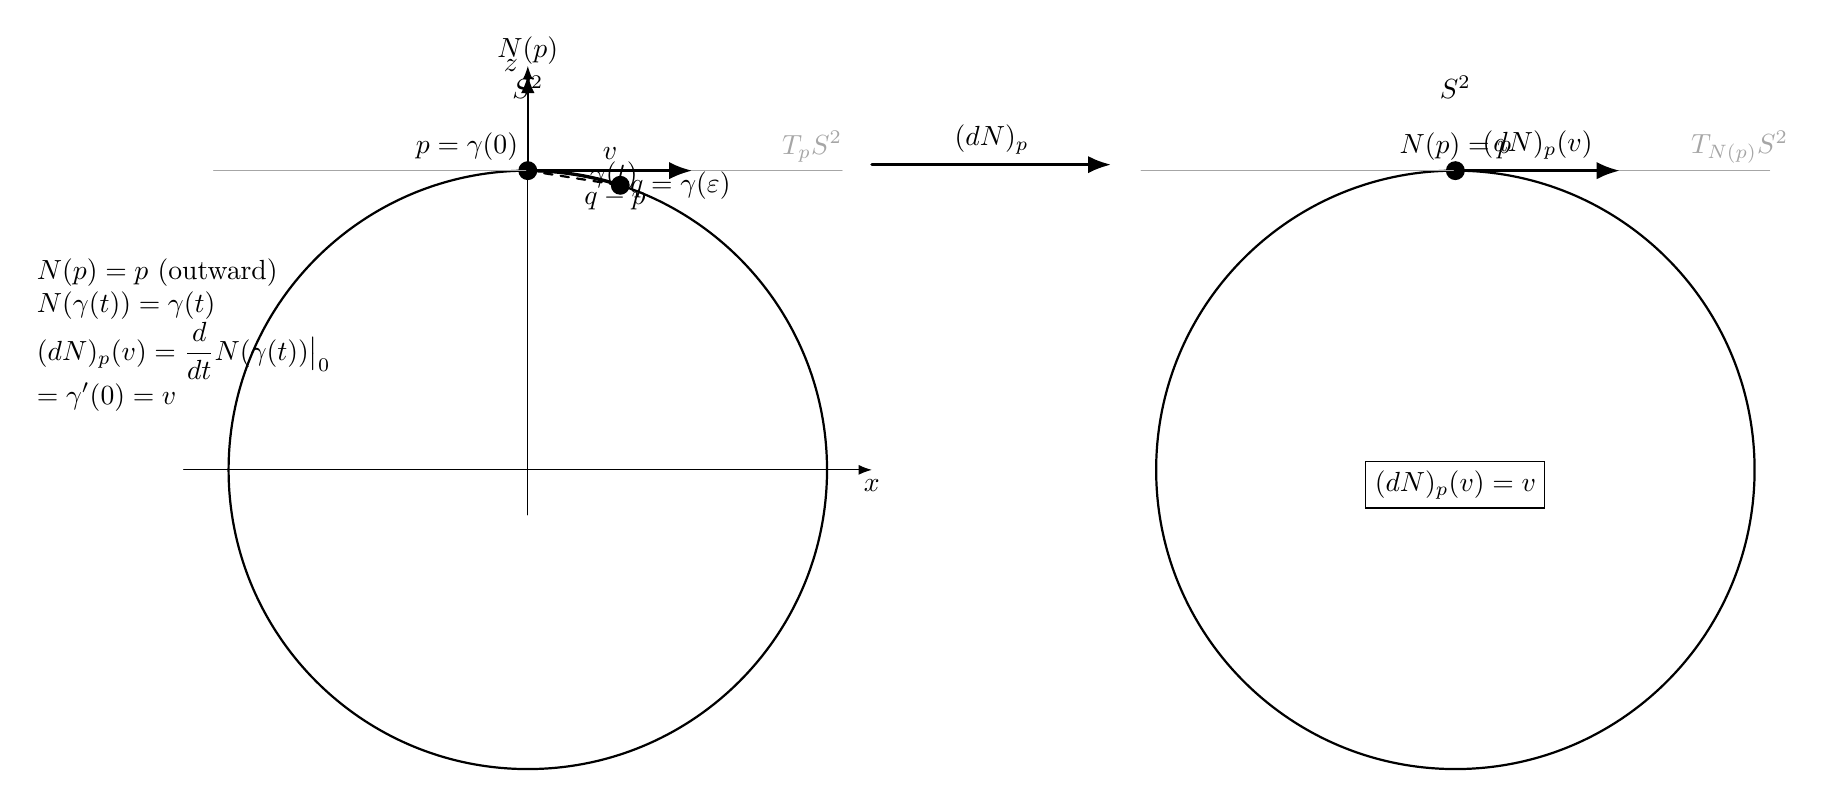
\begin{tikzpicture}[>=Latex, line cap=round, line join=round, scale=3.8]
		
		% Choose a concrete small step epsilon for a finite-difference picture
		\def\epsdeg{18}
		\pgfmathsetmacro{\sE}{sin(\epsdeg)}
		\pgfmathsetmacro{\cE}{cos(\epsdeg)}
		\pgfmathsetmacro{\epsrad}{\epsdeg*pi/180}
		
		% Left: S^2 with curve gamma(t) and v at p
		\begin{scope}[shift={(0,0)}]
			\draw[thick] (0,0) circle (1);
			\node at (0,1.28) {$S^2$};
			
			% axes
			\draw[->] (-1.15,0) -- (1.15,0) node[below] {$x$};
			\draw[->] (0,-0.15) -- (0,1.35) node[left] {$z$};
			
			% points p and q = gamma(eps)
			\coordinate (p) at (0,1);
			\coordinate (q) at (\sE,\cE);
			\fill (p) circle (0.9pt) node[above left] {$p=\gamma(0)$};
			\fill (q) circle (0.9pt) node[right] {$q=\gamma(\varepsilon)$};
			
			% curve gamma(t) = (sin t, cos t) in cross-section (y=0)
			\draw[very thick]
			(p) arc[start angle=90, end angle=90-\epsdeg, radius=1]
			node[pos=0.55, right] {$\gamma(t)$};
			
			% tangent line at p (horizontal)
			\draw[gray!70] (-1.05,1) -- (1.05,1);
			\node[gray!70] at (0.95,1.08) {$T_pS^2$};
			
			% tangent vector v = gamma'(0) = (1,0,0)  (drawn as (1,0) in cross-section)
			\draw[very thick,->] (p) -- ++(0.55,0) node[midway, above] {$v$};
			
			% normal at p : N(p)=p
			\draw[thick,->] (p) -- ++(0,0.32) node[above] {$N(p)$};
			
			% chord q-p for finite difference N(q)-N(p)=q-p (since N=Id)
			\draw[thick,dashed] (p) -- (q) node[midway, below right] {$q-p$};
			
			% label the finite difference quotient (schematic)
			\node[align=left] at (-1.15,0.45) {%
				$\displaystyle N(p)=p$ (outward)\\
				$\displaystyle N(\gamma(t))=\gamma(t)$\\
				$\displaystyle (dN)_p(v)=\frac{d}{dt}N(\gamma(t))\big|_{0}$\\
				$\displaystyle =\gamma'(0)=v$};
		\end{scope}
		
		% Right: Codomain tangent space at N(p)=p (same plane)
		\begin{scope}[shift={(3.1,0)}]
			\draw[thick] (0,0) circle (1);
			\node at (0,1.28) {$S^2$};
			
			% point N(p)=p at top
			\coordinate (np) at (0,1);
			\fill (np) circle (0.9pt) node[above] {$N(p)=p$};
			
			% tangent line at N(p) (horizontal)
			\draw[gray!70] (-1.05,1) -- (1.05,1);
			\node[gray!70] at (0.95,1.08) {$T_{N(p)}S^2$};
			
			% show (dN)_p(v) = v
			\draw[very thick,->] (np) -- ++(0.55,0) node[midway, above] {$(dN)_p(v)$};
			\node[align=center] at (0,-0.05) {$\boxed{(dN)_p(v)=v}$};
		\end{scope}
		
		% arrow indicating the differential map
		\draw[very thick,->] (1.15,1.02) -- (1.95,1.02) node[midway, above] {$(dN)_p$};
		
	\end{tikzpicture}
	
	\vspace{10pt}
	
	% ============================================================
	% (3) Shape operator S_p = -(dN)_p : T_p S^2 -> T_p S^2, S_p(v)=-v
	% ============================================================
	\begin{tikzpicture}[>=Latex, line cap=round, line join=round, scale=3.8]
		
		% Left: tangent plane at p and vectors v, S_p(v)
		\begin{scope}[shift={(0,0)}]
			\draw[thick] (0,0) circle (1);
			\node at (0,1.28) {$S^2$};
			
			% axes
			\draw[->] (-1.15,0) -- (1.15,0) node[below] {$x$};
			\draw[->] (0,-0.15) -- (0,1.35) node[left] {$z$};
			
			% point p
			\coordinate (p) at (0,1);
			\fill (p) circle (0.9pt) node[above left] {$p$};
			
			% tangent line at p
			\draw[gray!70] (-1.05,1) -- (1.05,1);
			\node[gray!70] at (0.95,1.08) {$T_pS^2$};
			
			% normal N(p)
			\draw[thick,->] (p) -- ++(0,0.32) node[above] {$N(p)$};
			
			% v and -v
			\draw[very thick,->] (p) -- ++(0.55,0) node[midway, above] {$v$};
			\draw[very thick,->] (p) -- ++(-0.55,0) node[midway, above] {$-v$};
			
			% shape operator formula
			\node[align=left] at (-1.15,0.48) {%
				$\displaystyle S_p:T_pS^2\to T_pS^2$\\
				$\displaystyle S_p(v)=-(dN)_p(v)$\\
				$\displaystyle (dN)_p(v)=v\ \Rightarrow\ \boxed{S_p(v)=-v}$};
		\end{scope}
		
		% Right: matrix in a chosen basis (diagonal form)
		\begin{scope}[shift={(3.1,0)}]
			% Draw a coordinate plane for T_pS^2 with basis e1,e2
			\node at (0,1.28) {$T_pS^2$ with basis};
			
			% basis vectors in the tangent plane (schematic 2D)
			\coordinate (O) at (0,0.25);
			\draw[->] (O) -- ++(1.0,0) node[below right] {$e_1$};
			\draw[->] (O) -- ++(0,1.0) node[above left] {$e_2$};
			
			% show action of S_p on basis (scaling by -1)
			\draw[very thick,->] (O) -- ++(-0.75,0) node[below left] {$S_p(e_1)=-e_1$};
			\draw[very thick,->] (O) -- ++(0,-0.75) node[below] {$S_p(e_2)=-e_2$};
			
			% matrix
			\node[align=center] at (0,0.95) {$\displaystyle [S_p]_{\{e_1,e_2\}}
				=\begin{pmatrix}-1&0\\[2pt]0&-1\end{pmatrix}$};
			
			\node[align=center] at (0,-0.05) {\(\displaystyle\boxed{S_p=-\mathrm{Id}}\)};
		\end{scope}
		
		% arrow emphasizing "choose a basis -> diagonal"
		\draw[very thick,->] (1.15,1.02) -- (1.95,1.02)
		node[midway, above] {choose basis \(\{e_1,e_2\}\)};
		
	\end{tikzpicture}
	
\end{document}
